\documentclass{article}
\usepackage{graphicx} % Required for inserting images
\usepackage{booktabs} % For better table formatting
\usepackage{array}    % For more flexible table features
\usepackage{placeins} % To control figure placement
\usepackage{float}    % To use the H placement specifier

\title{Analysis of Single Mutants}
\author{Your Name} % Replace with your name
\date{}

\begin{document}

\maketitle

\section*{Introduction}
To guide the selection of mutations for directed evolution, a multiple sequence alignment was performed between the human and mouse wild-type protein. This MSA revealed 47 positions that differed between the human and mouse sequences, suggesting potential sites for mutagenesis. In order to prioritize residues for mutagenesis, the distances from the alpha carbon of Cys/Sec49 (active site residue) and the rest of the 46 positions were calculated. Residues were then grouped into distance criteria of <10 Å, 10-15 Å, 15-20 Å, 20-25 Å, 25-30 Å, and 30-35 Å. This distance-based approach allowed us to select residues within different proximity ranges to Cys/Sec49. Grouping residues into distance bins provides a systematic and stochastic way to explore the impact of mutations at varying distances from the target residue (Cys/Sec49). 

To investigate the individual contributions of each residue to the structural and functional differences between the human and mouse proteins, single mutants were generated systematically. Each mutation corresponds to substituting a residue in the mouse protein with its human counterpart, or vice versa, as outlined in the mutation table of 47 residues. This process was conducted one residue at a time to isolate the effects of each mutation.

The mutations were applied by transferring each residue from the mouse sequence to the human sequence and vice versa, ensuring a controlled and systematic approach to mutagenesis. The active site residue, Cys/Sec49, remained a fixed reference point, with all mutations being calculated relative to it. For example, residues such as position 3 (N to K) and position 4 (R to S) involved changes in side-chain polarity or charge, while others, such as position 48 (Y to F), focused on aromatic substitutions. These single-residue changes allow for direct comparisons of the energetic and structural effects of each mutation, enabling us to study how these variations influence activation barriers and overall protein function.

By analyzing the 47 single mutants, we aim to systematically explore the structural transitions and activation energy changes associated with the human-to-mouse and mouse-to-human sequence transformations. This stepwise approach ensures that the contributions of individual residues to protein evolution and function are thoroughly characterized.

\begin{figure}[H]
    \centering
    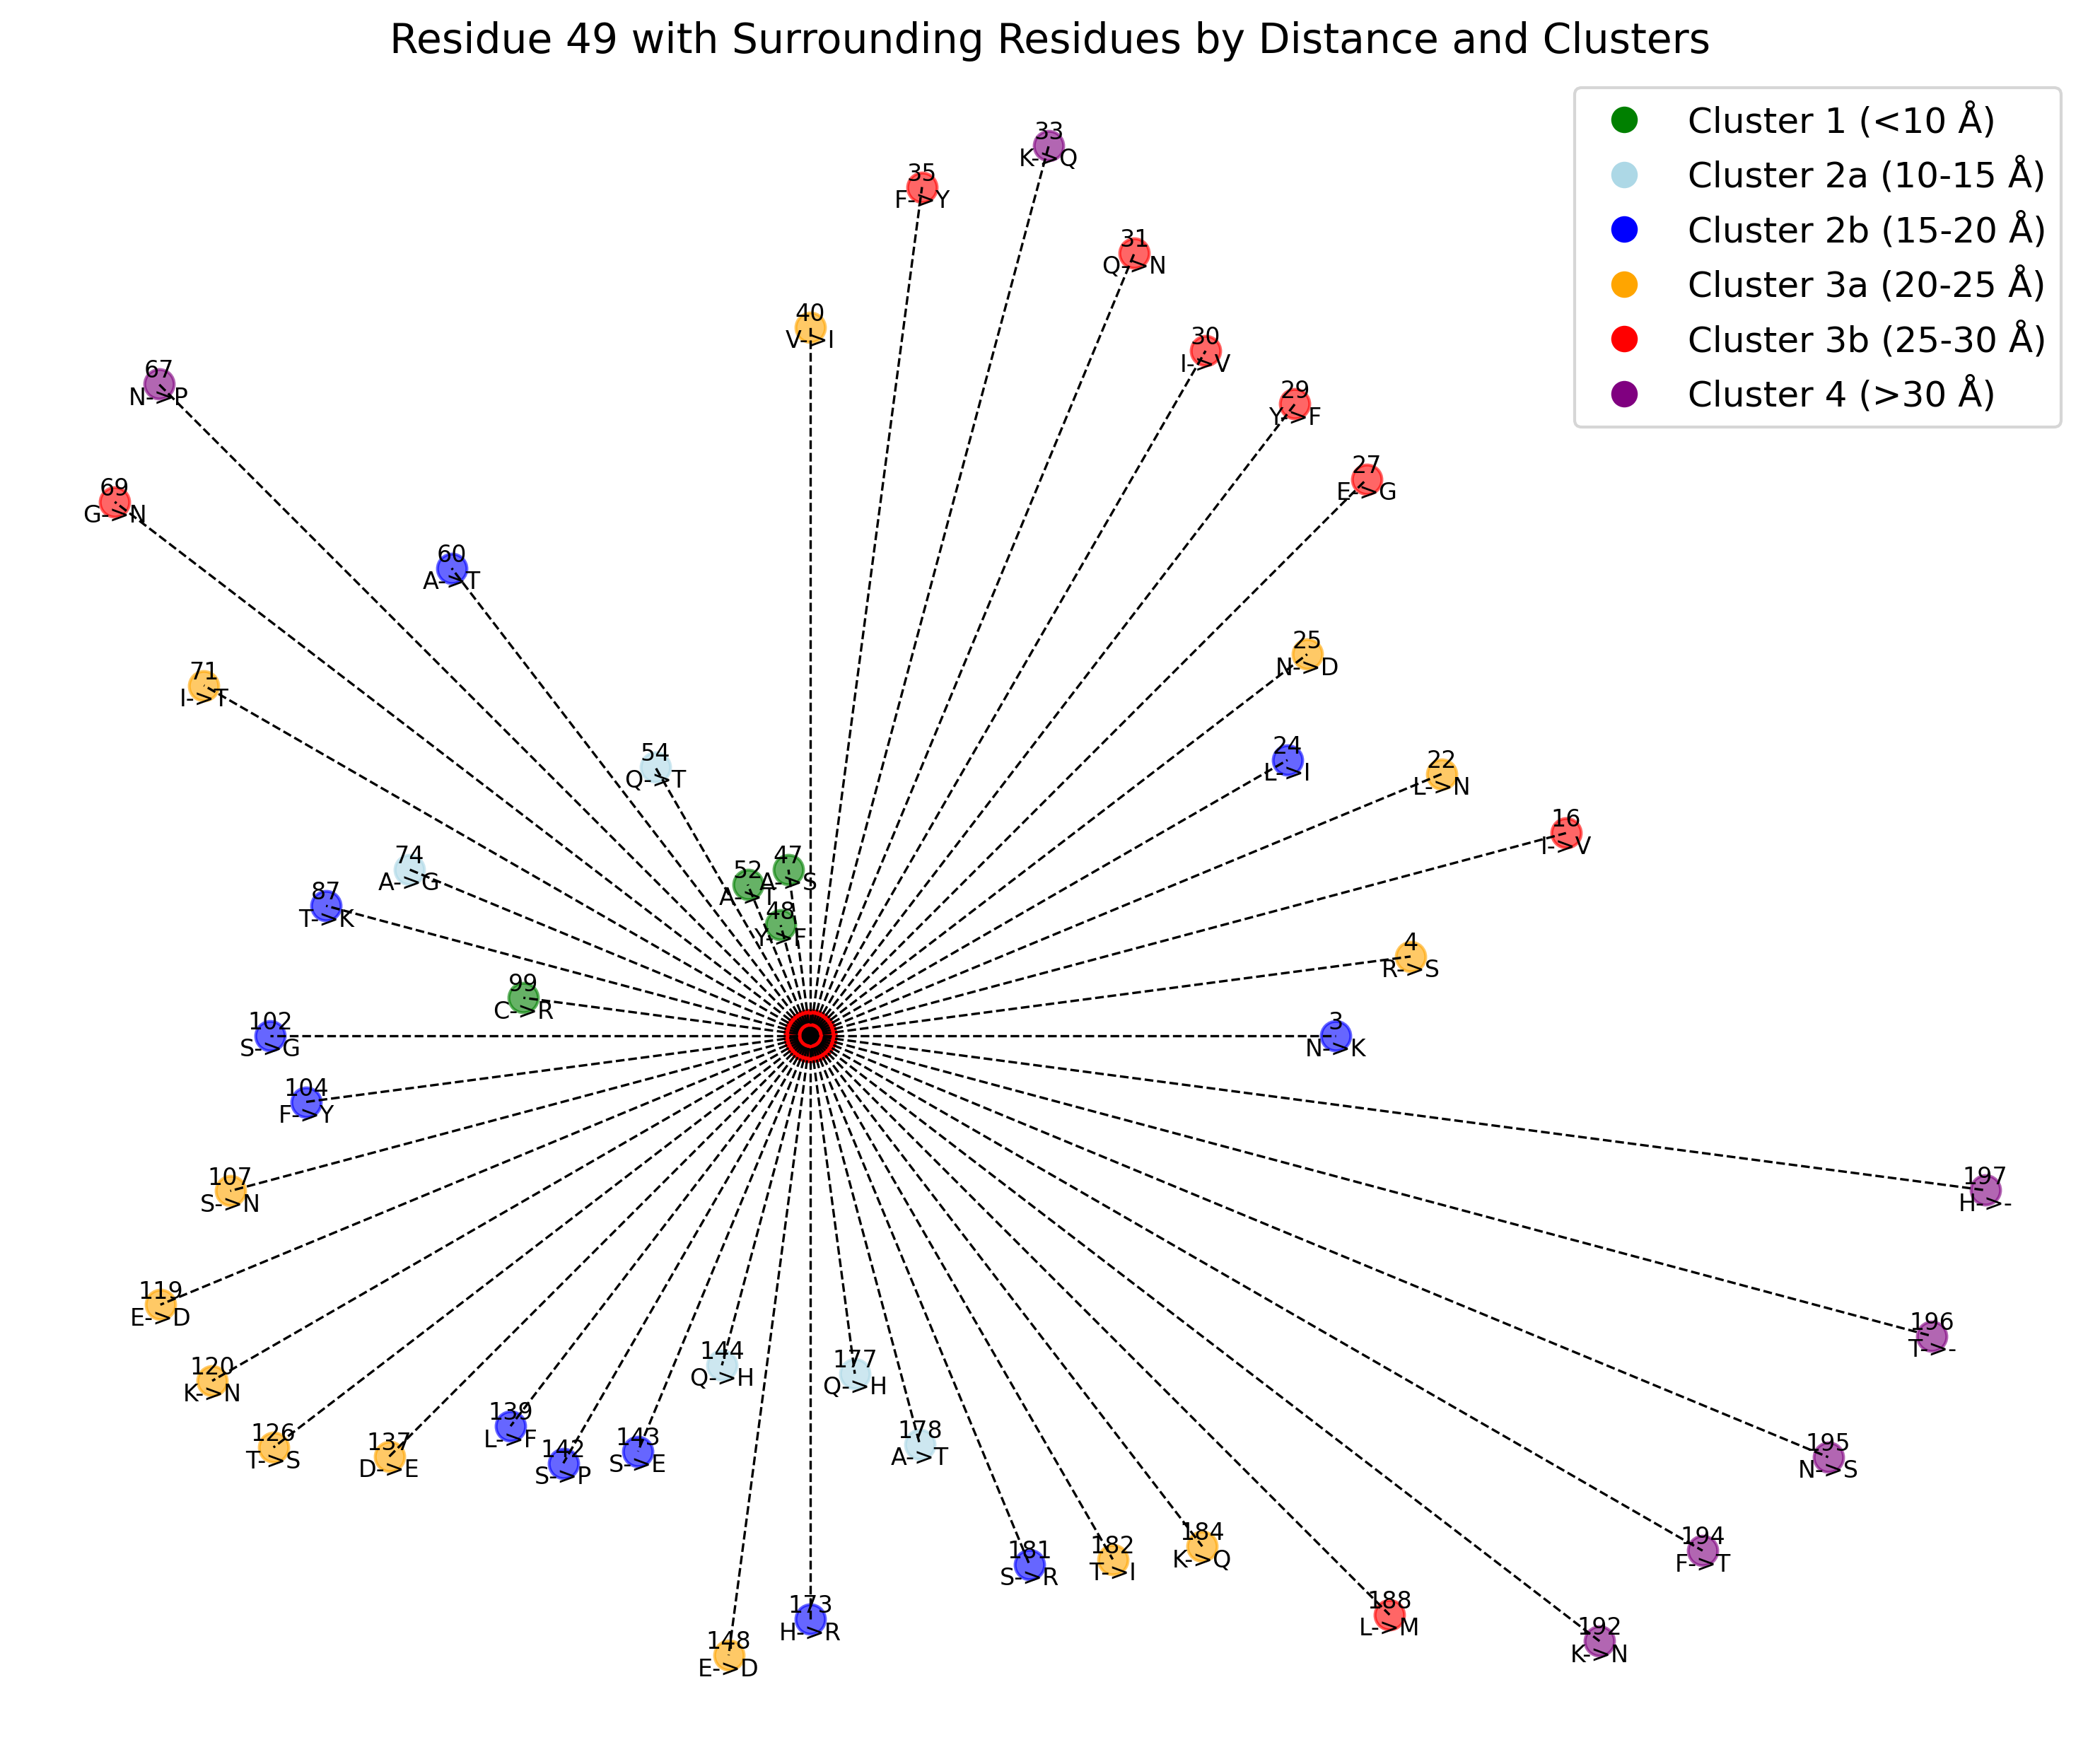
\includegraphics[width=0.8\linewidth]{/home/hp/nayanika/github/GPX6/figures/Residue_human_Distances.png} % Replace with your image file name
    \caption{Distance of residues from the active site for human mutants. The figure highlights proximity of each residue to Cys/Sec49.}
    \label{fig:human_distances}
\end{figure}

\begin{figure}[H]
    \centering
    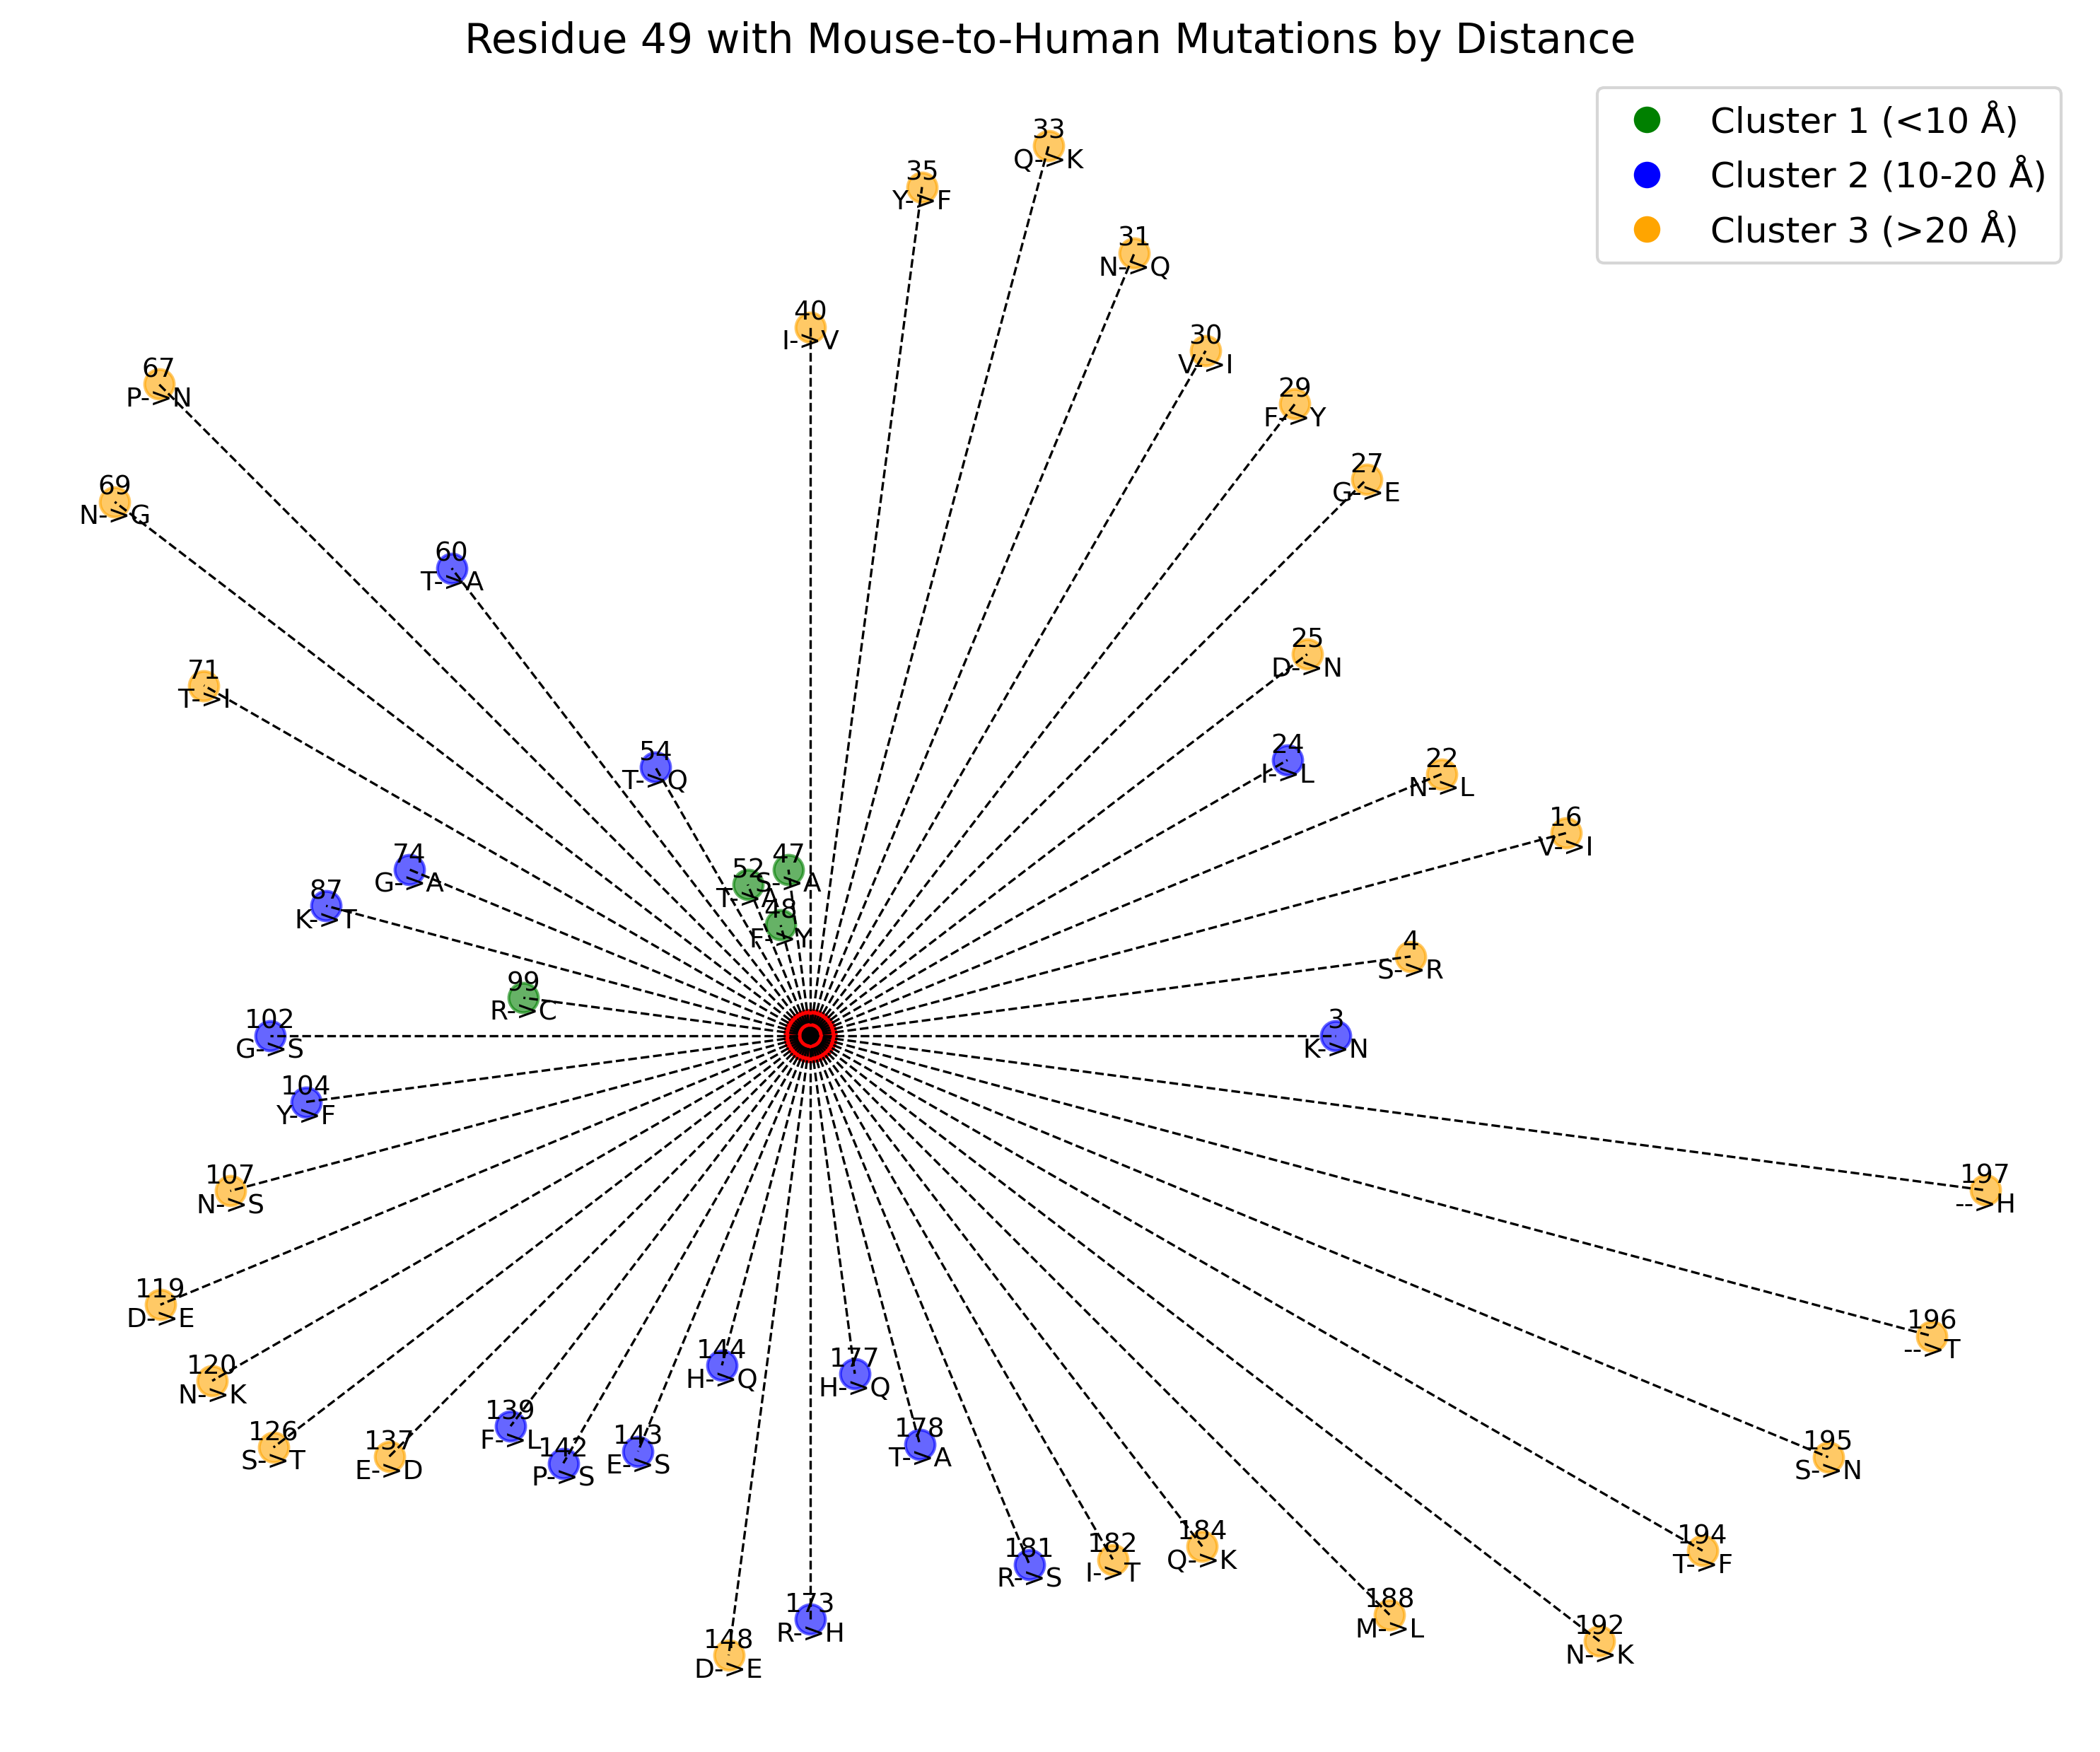
\includegraphics[width=0.8\linewidth]{/home/hp/nayanika/github/GPX6/figures/Residue_mouse_Distances.png} % Replace with your image file name
    \caption{Distance of residues from the active site for mouse mutants. The figure highlights proximity of each residue to Cys/Sec49.}
    \label{fig:mouse_distances}
\end{figure}

\FloatBarrier % Forces all previous figures to appear before this section

\subsection{Clustering the Variants}

The image below shows a 3D scatter plot of residues clustered based on their spatial proximity, hydrophobicity, and free energy values. The analysis begins by extracting residue data from a PDB file, where each residue’s position and amino acid identity are mapped. The residues are represented by their 3D coordinates, which are then used to compute pairwise distances. These distances are input into the KMeans clustering algorithm to group residues spatially, with the optimal number of clusters determined using the Elbow Method.

Residues are color-coded based on their **hydrophobicity** (a physicochemical property) to highlight how the hydrophobicity influences the clustering. The clustering provides insight into spatial relationships and physicochemical properties that might play a role in protein function.

Cluster 0: (P, E, H at positions 142-144)
    • Residues: Proline (P), Glutamic acid (E), Histidine (H)
    • Interpretation: These residues form a structural region, and their proximity to Cys/Sec49 is relatively far (16.44, 15.29, and 11.60 Å). 
Cluster 1: (V, Q, Y at positions 16, 33, 35)
    • Residues: Valine (V), Glutamine (Q), Tyrosine (Y)
    • Interpretation: These residues are located at a distance of 27.12, 30.54, and 28.03 Å from Cys/Sec49, respectively.
Cluster 2: (R, I, Q, M at positions 181-188)
    • Residues: Arginine (R), Isoleucine (I), Glutamine (Q), Methionine (M)
    • Interpretation: These residues are located further away from the active site, with distances ranging from 19.54 Å to 27.64 Å. 
Cluster 3: (S, F, R at positions 47, 48, 99)
    • Residues: Serine (S), Phenylalanine (F), Arginine (R)
    • Interpretation: These residues are closer to the active site, with distances ranging from 5.59 to 9.50 Å. This suggests they have a more direct influence on the active site. 
Cluster 4: (N, T, S at positions 192-195)
    • Residues: Asparagine (N), Threonine (T), Serine (S)
    • Interpretation: These residues are at relatively greater distances from Cys/Sec49, with distances ranging from 33.41 to 35.43 Å. 
Cluster 5: (D, N, S, D at positions 119, 120, 126, 148)
    • Residues: Aspartic acid (D), Asparagine (N), Serine (S)
    • Interpretation: These residues are located between 16.44 and 23.30 Å from Cys/Sec49. 
Cluster 6: (H, T at positions 177-178)
    • Residues: Histidine (H), Threonine (T)
    • Interpretation: The distances between these residues and Cys/Sec49 are 20.19 and 14.81 Å.
Cluster 7: (I, D, G at positions 24-27)
    • Residues: Isoleucine (I), Aspartic acid (D), Glycine (G)
    • Interpretation: These residues are further away from the active site, with distances ranging from 18.69 to 26.67 Å.
Cluster 8: (I, T at positions 40, 71)
    • Residues: Isoleucine (I), Threonine (T)
    • Interpretation: With distances of 23.17 and 23.11 Å from Cys/Sec49.
Cluster 9: (K, S at positions 3, 4)
    • Residues: Lysine (K), Serine (S)
    • Interpretation: These residues are 21.63 and 19.64 Å from Cys/Sec49. 
Cluster 10: (T, T at positions 52, 54)
    • Residues: Threonine (T)
    • Interpretation: The two Threonine residues at distances of 5.20 and 10.00 Å from Cys/Sec49 are relatively close. 
Cluster 11: (E, F at positions 137, 139)
    • Residues: Glutamic acid (E), Phenylalanine (F)
    • Interpretation: These residues are situated at distances of 21.60 and 16.28 Å, which are moderate. 
Cluster 12: (G at position 102)
    • Residue: Glycine (G)
    • Interpretation: Glycine is located at a distance of 16.77 Å
Cluster 13: (P, N at positions 67, 69)
    • Residues: Proline (P), Asparagine (N)
    • Interpretation: With distances of 30.74 and 27.97 Å
Cluster 14: (T, N at positions 60, 107)
    • Residues: Threonine (T), Asparagine (N)
    • Interpretation: With distances ranging from 19.05 to 19.80 Å
Cluster 15: (N, F, V, N at positions 22-31)
    • Residues: Asparagine (N), Phenylalanine (F), Valine (V)
    • Interpretation: These residues are 22.91, 26.66, and 28.12 Å from Cys/Sec49
Cluster 16: (G at position 74)
    • Residue: Glycine (G)
    • Interpretation: Glycine at 14.29 Å 
Cluster 17: (R at position 173)
    • Residue: Arginine (R)
    • Interpretation: Arginine at 20.19 Å 
Cluster 18: (Y at position 104)
    • Residue: Tyrosine (Y)
    • Interpretation: Tyrosine at 16.10 Å 
Cluster 19: (K at position 87)
    • Residue: Lysine (K)
    • Interpretation: Lysine at 16.44 Å 

    Cluster 0: (P, E, H at positions 142-144)
    • Residues: Proline (P), Glutamic acid (E), Histidine (H)
    • Interpretation: These residues may form a specific structural region with a mix of hydrophobic (Proline) and polar (Glutamic acid, Histidine) properties. 
    • Residues: Valine (V), Glutamine (Q), Tyrosine (Y)
    • Interpretation: This cluster contains a hydrophobic residue (Valine) and polar residues (Glutamine, Tyrosine). 
Cluster 2: (R, I, Q, M at positions 181-188)
    • Residues: Arginine (R), Isoleucine (I), Glutamine (Q), Methionine (M)
    • Interpretation: This cluster is rich in charged (Arginine) and hydrophobic (Isoleucine, Methionine) residues
Cluster 3: (S, F, R at positions 47, 48, 99)
    • Residues: Serine (S), Phenylalanine (F), Arginine (R)
    • Interpretation: This cluster involves a polar residue (Serine), an aromatic residue (Phenylalanine), and a basic residue (Arginine).
Cluster 4: (N, T, S at positions 192-195)
    • Residues: Asparagine (N), Threonine (T), Serine (S)
    • Interpretation: The cluster contains polar residues
Cluster 5: (D, N, S, D at positions 119, 120, 126, 148)
    • Residues: Aspartic acid (D), Asparagine (N), Serine (S)
    • Interpretation: This cluster involves acidic (Aspartic acid) and polar (Serine, Asparagine) residues
Cluster 6: (H, T at positions 177-178)
    • Residues: Histidine (H), Threonine (T)
    • Interpretation: This small cluster of polar residues 
Cluster 7: (I, D, G at positions 24-27)
    • Residues: Isoleucine (I), Aspartic acid (D), Glycine (G)
    • Interpretation: A mix of hydrophobic (Isoleucine) and polar (Aspartic acid) residues, with Glycine 
Cluster 8: (I, T at positions 40, 71)
    • Residues: Isoleucine (I), Threonine (T)
    • Interpretation: The hydrophobic Isoleucine and polar Threonine residues
Cluster 9: (K, S at positions 3, 4)
    • Residues: Lysine (K), Serine (S)
    • Interpretation: The charged Lysine and polar Serine residues
Cluster 10: (T, T at positions 52, 54)
    • Residues: Threonine (T)
    • Interpretation: This cluster consists of two Threonine residues
Cluster 11: (E, F at positions 137, 139)
    • Residues: Glutamic acid (E), Phenylalanine (F)
    • Interpretation: This cluster involves a charged (Glutamic acid) and aromatic (Phenylalanine) residue
Cluster 14: (T, N at positions 60, 107)
    • Residues: Threonine (T), Asparagine (N)
    • Interpretation: A cluster of polar residues l
Cluster 15: (N, F, V, N at positions 22-31)
    • Residues: Asparagine (N), Phenylalanine (F), Valine (V)
    • Interpretation: The combination of polar (Asparagine) and hydrophobic (Phenylalanine, Valine) residues 


\begin{figure}[H]
    \centering
    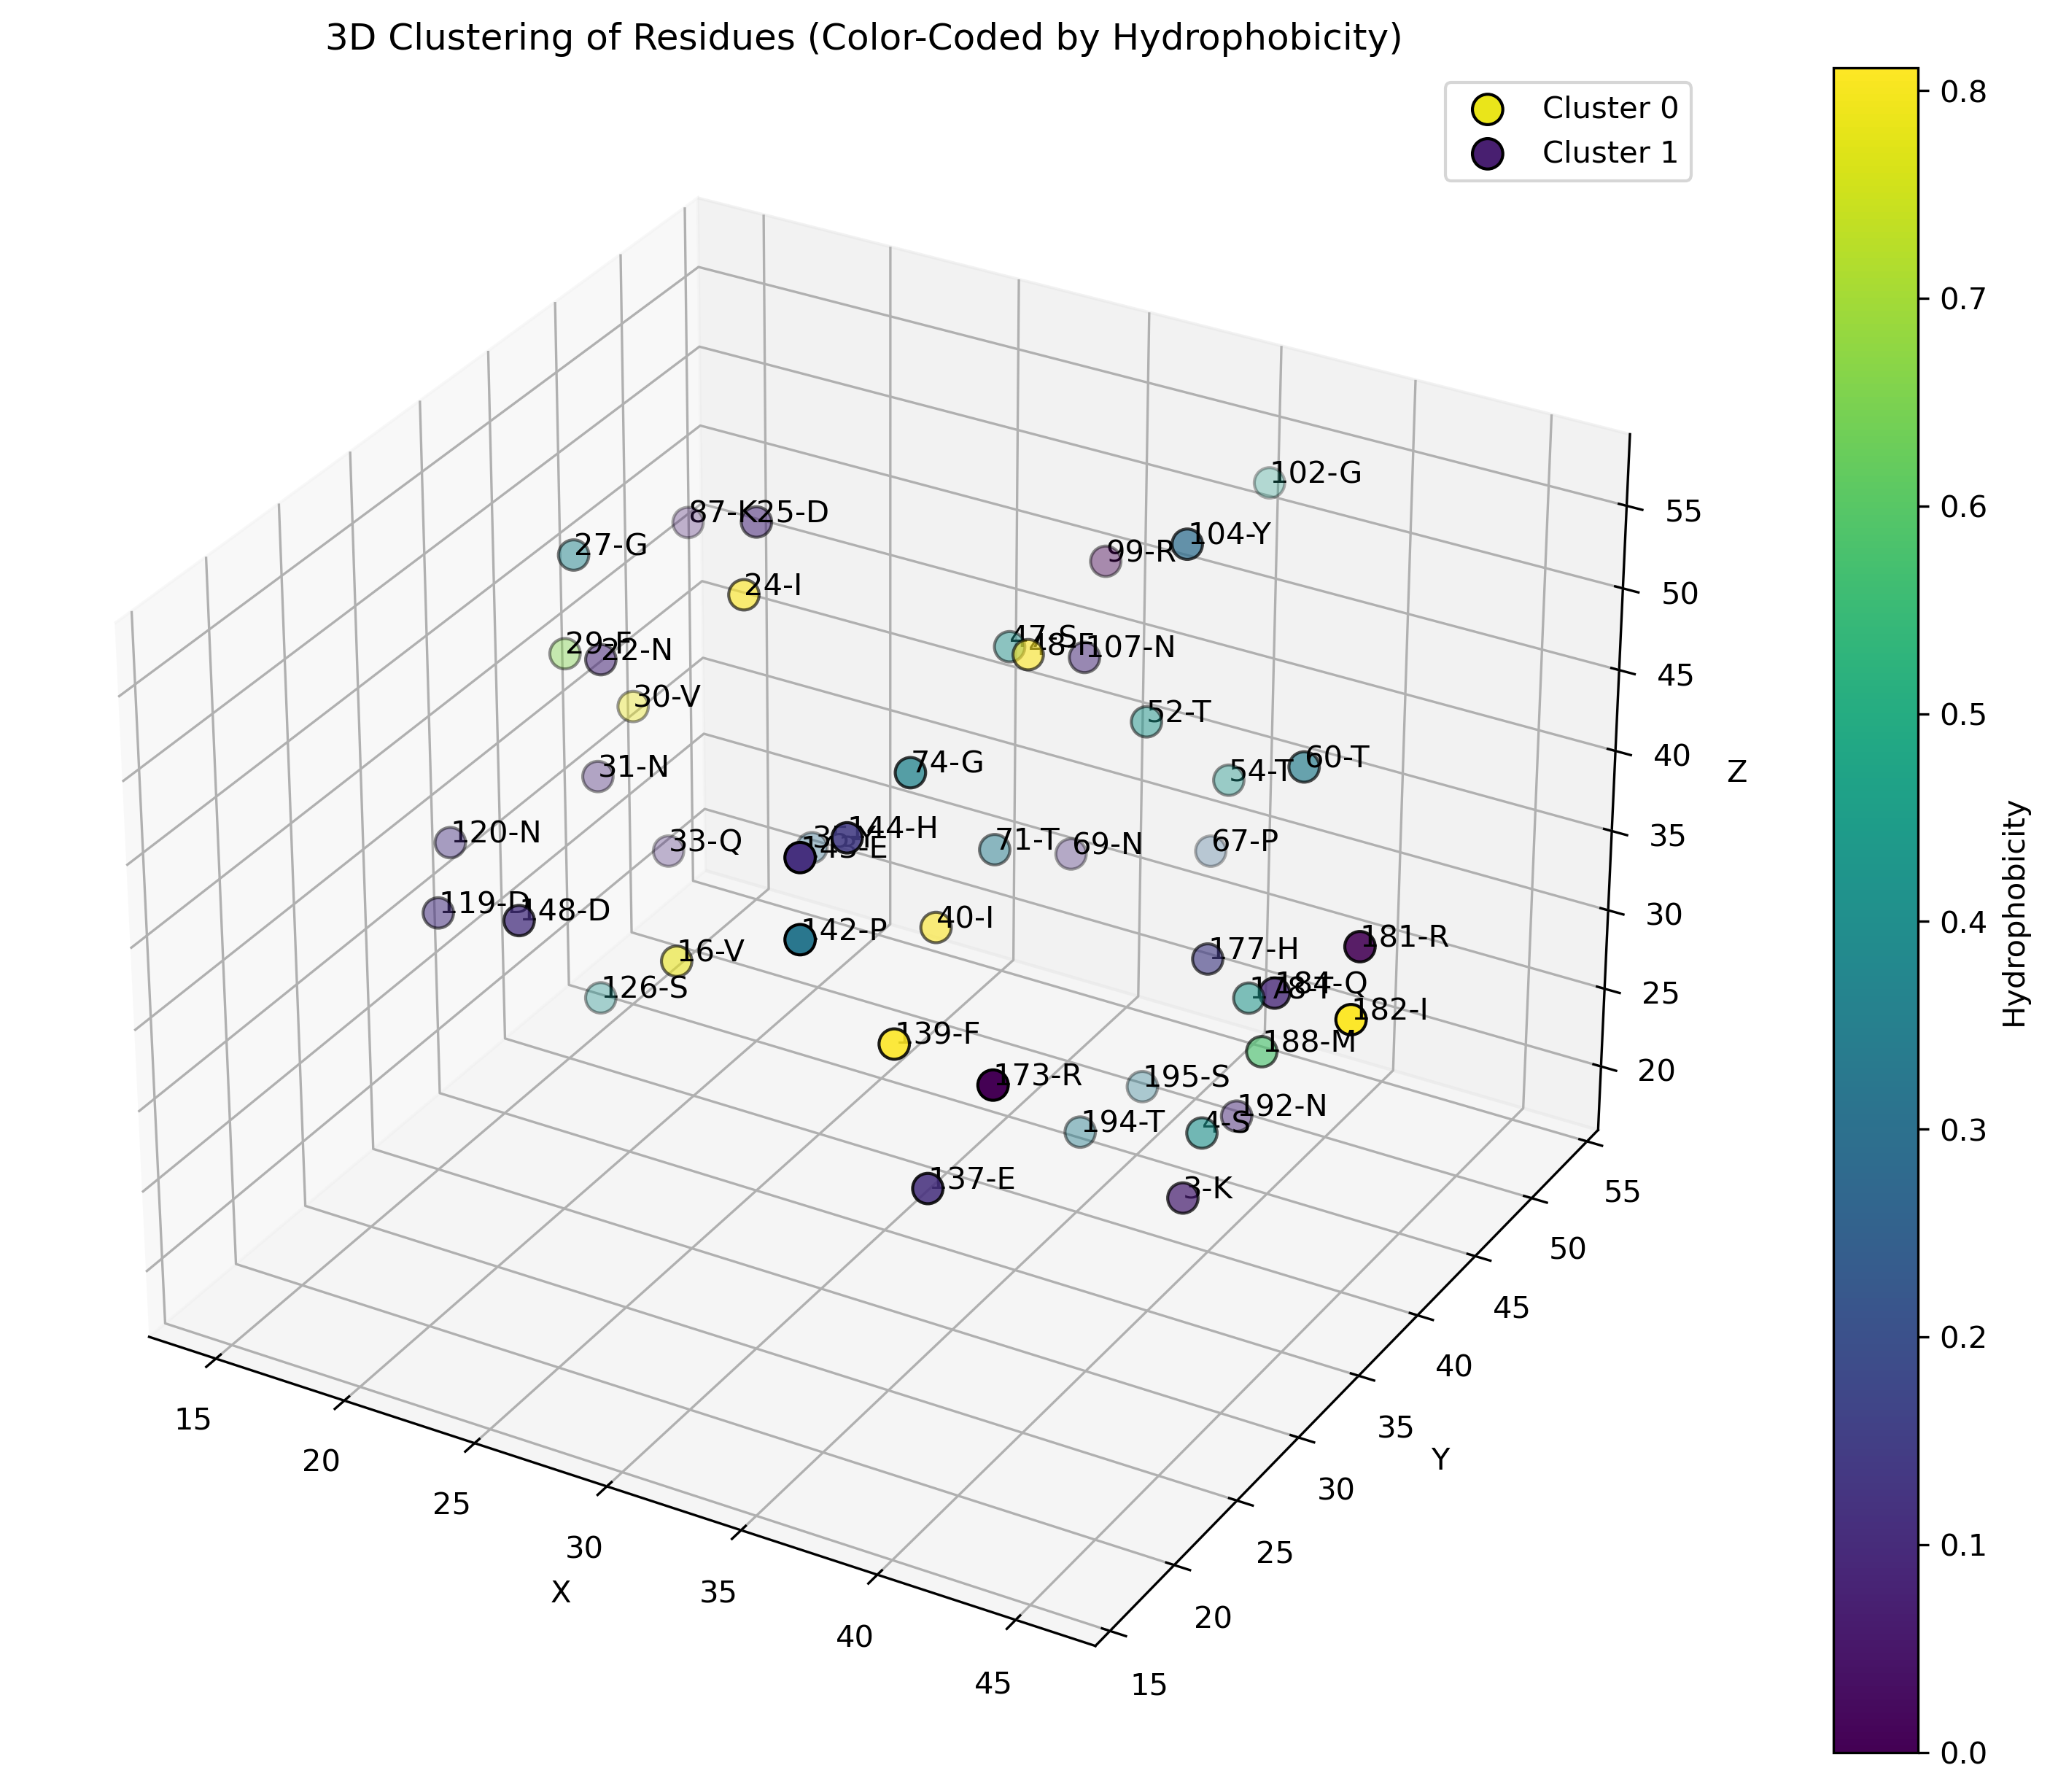
\includegraphics[width=0.8\linewidth]{/home/hp/nayanika/github/GPX6/figures/3d_clustering_residues.png} % Replace with your image file name
    \caption{3D clustering of residues based on spatial proximity, hydrophobicity, and free energy values. Each cluster represents residues grouped by their spatial location and physicochemical properties.}
    \label{fig:3d_clustering}
\end{figure}

\FloatBarrier % Forces all previous figures to appear before this section

\subsection{Visualizing the Clusters}

The following figure illustrates the clustering of mutants based on the distances from the active site and other relevant features. This visualization provides a clear representation of how mutations at different positions affect the protein’s structure and potential function.

\begin{figure}[H]
    \centering
    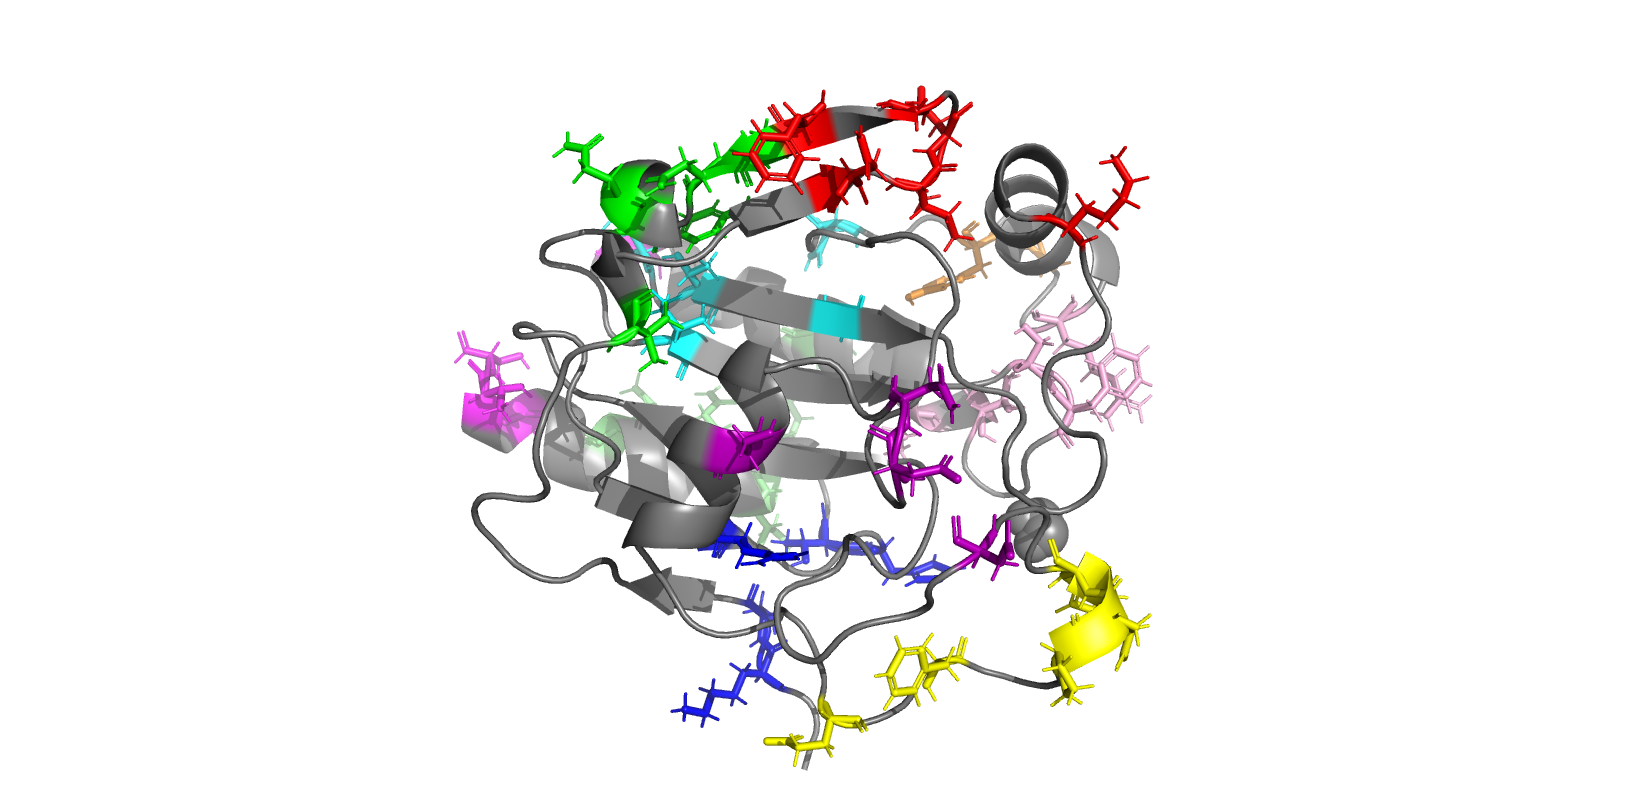
\includegraphics[width=0.8\linewidth]{/home/hp/nayanika/github/GPX6/figures/clustered_mutants.png} % Replace with your image file name
    \caption{Visualization of clustered mutants showing the proximity of residues to Cys/Sec49.}
    \label{fig:clustered_mutants}
\end{figure}

\end{document}
